\documentclass[a4paper]{article}
\usepackage[utf8]{inputenc}
\usepackage[T1]{fontenc}
\usepackage{url}
\usepackage{tikz}
\usepackage{csvsimple}
\usepackage[]{algorithm2e}

\title{2-24-1 Optimization and search heuristics}
\author{Baptiste Louf, Yann Ramusat}

\begin{document}
\maketitle

%For the purpose of the project we have implemented most of the algorithms seen during the first part of the course.
%In addition to the \textit{RLS} and \textit{(1+1)EA} that are already part of the bootstrap project we propose the \textit{($\mu$+$\lambda$)EA}, the \textit{($\mu$,$\lambda$)EA}, the \textit{simulated annealing} and the \textit{1+($\lambda$,$\lambda$)GA}.
%
%We also use an heuristic to identify useless object and delete them. You can find more information for this processing in INSERT REF.
%
%We will discuss about the impact of the preprocessing, the optimal parameters $\lambda$ and $\mu$ for each algorithm and we will compare the differents heuristics over different kind of instances.
%
%TODO PRECISE CONFIG OF THE PC.
%
%\tableofcontents
%
%\newpage
%
%\section{Preprocessing}
%
%We begin with a comparison of the effectiveness of the \textit{RLS} with and without the preprocessing. This will give an insight of the utility of this method. We consider the dataset \textbf{fnl4461 n4460 bounded-strongly-corr 01}.
%
%\begin{figure}[!h]
%	\begin{center}
%		\begin{tikzpicture}[scale = 0.6]
%			\draw[step=1,gray,thin]  (0,0) grid (7,7);
%			\foreach \x in {.5,1.0,1.5,2.0,2.5,3.0,3.5,4.0}
%		 \node[anchor=north] at (2*\x-1,0) {\x};
%			\foreach \y in {1,2,3,4,5,6}
%		 \node[anchor=east] at (0,\y) {\y};
%			\draw (3.4,-1.2) node{Duration time $1\cdot10^3$ ms};
%			\draw (-1.3,3.5) node[rotate=90]{Objective $3.33\cdot10^5$};
%			
%			\draw[thick] plot[mark=*]  file {with_preproc.txt};
%			\draw[thick, color=gray] plot[mark=+] file {no_preproc.txt};
%			
%			\draw[white] (13,6)node[fill=black!80] {With preprocessing};
%			\draw(13,5)node[fill=gray!50] {No preprocessing};
%		\end{tikzpicture}
%	\end{center}
%	\caption{Effectiveness with and without preprocessing.}
%	\label{expe_preprocessing}
%\end{figure}
%
%This suggests the preprocessing is not so usefull. In the following tests we will assume the preprocessing is desactivated.
%
%\section{Finding optimal parameters}
%
%We now search for optimal values for the parameters given to the \textit{Evolutionary Algorithms}.
%
%\subsection{Parameters for the ($\mu$+$\lambda$)EA}
%
%We have computed results over the same dataset as before but with a time limit fixed to $2$ seconds.
%
%In the following table we give the objective value ($\cdot 10^3$) depending on $\lambda$ (columns) and $\mu$ (rows). 
%
%\begin{center}
%\csvautotabular{mu+lambda.csv}
%\end{center}
%
%
%We do not represent greater values of $\mu$ because they are worth.
%
%We observe that definitively, the best value for $\mu$ is $1$ and that $\lambda$ can be taken around $5$ or $6$.
%
%
%\subsection{Parameters for the ($\mu$,$\lambda$)EA}
%
%We still use the same dataset and the same time limit.
%
%\begin{center}
%\csvautotabular{mu-lambda.csv}
%\end{center}
%
%For the two algorithm the impact of the values are similar (except when $\mu$ and $\lambda$ are equals to 1).
%
%We conclude optimal parameters are $1$ for $\mu$ and around $10$ for $\lambda$.
%
%\section{Comparisons between algorithms over different datasets}
%
%\subsection{Optimum reached}
%
%\begin{center}
%\csvautotabular{a280.csv}
%\end{center}
%
%\begin{center}
%\csvautotabular{fnl4461.csv}
%\end{center}
%
%\begin{center}
%\csvautotabular{pla33810.csv}
%\end{center}
%
%\subsection{Convergence}

\section{Outline of the algorithm(s) and choices made}
\begin{algorithm}
\KwData{An instance}
 \KwResult{A tour and its objective value}
	Find a TSP tour\;
	\textit{** Preprocessing **}\;
\While{not over}{
  mutate current solution\;
  \If{improved condition satisfied}{
   update solution\;
   }
  }
  return solution\;
 \caption{outline of the algorithm}
\end{algorithm}
\subsection{Finding the tour}
A critical issue in the TTP problem is finding a nice tour. Indeed, according to the packing plan one chooses, the optimal tour may vary, and conversely. In the original paper, the choice is made to compute a good solution for TSP, and then fix the tour forever and focus on the packing plan. We made the same choice.\\
We could have computed a "good tour" ourselves, considering that taking a TSP solution does not take into account the fact that the bag gets heavier over time, and thus smaller distances should be traveled at the end of the journey. However, efficient algorithms for TSP are already quite complicated, so we had no chance to find a good algorithm for that slightly different problem, and it seems beyond the point of a search heuristics project. Nonetheless, this raises a nice research question that we leave open.\\
Another possibility was to use the precomputed tour as a starting point, and then do some local mutations (for instance : choose two consecutive cities in the tour and swap them). There were two options :\\
- take a tour, optimize the packing plan for that tour, mutate the tour, optimize the packing plan for the mutated tour, compare, and start again … This would mean one optimization problem inside another, and would be time consuming\\
- mutate the tour and the packing plan at the same time. This would result in a huge search space, we decided not to try.
\subsection{Preprocessing the instance}
In the original paper, there is an algorithm called Simple Heuristic, that takes into account the particularities of the problem. The results show that it is very inefficient compared to search algorithms, but there is a smart step in that simple heuristic where they discard \textit{disadvantageous} items : a simple condition tells if in any situation, the packing plan with that object is worse than the packing plan without that object. In that situtation we could preprocess the instance by removing all \textit{disadvantageous} items.\\
However, the improvement was not substantial, and vanishes asymptotically, so we dropped that idea, especially since we want to avoid overfitting.

\subsection{Search Heuristics}
We considered 6 different kinds of heuristics : random local search, simulated annealing, the ($\mu$+$\lambda$) EA, the ($\mu$,$\lambda$) EA, the 1+($\lambda$,$\lambda$) GA and a search heuristics that randomly chooses mutations at each step.
\subsubsection{Simulated annealing}
Simulated annealing is almost the same as RLS, except that at each step, is the mutated solution is worse, there is a small probability of keeping it, i.e. if the mutated solution is at distance $d$ to the best solution seen so far, we keep it with probability $e^{-d\log(n)/100}$, where we are at step $n$.

\subsubsection{Finding $\mu$ and $\lambda$}
We ran preliminary tests on the ($\mu + \lambda$) EA : to determine the "best" values for $\mu$ and $\lambda$, on the default dataset with a runtime of $2$ seconds.

In the following table we give the objective value ($\cdot 10^3$) depending on $\lambda$ (columns) and $\mu$ (rows) (we don't include further values which are way worse). 

\begin{center}
\csvautotabular{mu+lambda.csv}
\end{center}

We did exactly the same for the ($\mu$,$\lambda$) EA :


\begin{center}
\csvautotabular{mu-lambda.csv}
\end{center}

Hence, for simplicity, we fixed $\mu=1$ and $\lambda=7$ for both algorithms.

\subsubsection{Considering several mutations}
The idea here is to, at each step, randomly choose one mutation and apply it to the current solution, then replace the current solution if it is improved. After some preliminary tests, we chose to mutate as RLS with probability $1/2$ and as ($\mu + \lambda$) w.p. $1/2$.
\section{Experimental results}
\subsection{Methodology}
We chose to test our heuristics on the 9 datasets of the CEC competition, as it would take too long to test on all the datasets we were provided with. It still covers the main differences in parameters (size, number of items, correlations, ettc.), and we are given benchmark objectives. \\
On every dataset, we ran each algorithm with a time limit of 10 minutes (as in the CEC competition), and the algorithm stops if 1000000 steps without improvement  were observed. The result is averaged over 3 runs of the algorithm.
\subsection{Results}
We obtain satisfying results : except for the hardest instance, our results are always slightly better than the objectives of the CEC competition, and we even have a much better result on the penultimate instance. The random mutation is the best on small and medium instances (it probably finds the global optimum on the small instances since it always returns the same value), but it is really slow to converge. The simulated annealing is by far the best on big instances. The RLS performs well on every instance, especially on big ones. The ($\mu + \lambda$) EA gives good results for small and medium instances. The 1+($\lambda$,$\lambda$) GA is also quite good on small and medium instances, and the worst algorithm here is the ($\mu$,$\lambda$) EA.

\begin{center}
\csvautotabular{a280.csv}
\end{center}

\begin{center}
\csvautotabular{fnl4461.csv}
\end{center}

\begin{center}
\csvautotabular{pla33810.csv}
\end{center}

\begin{figure}[!h]
	\begin{center}
		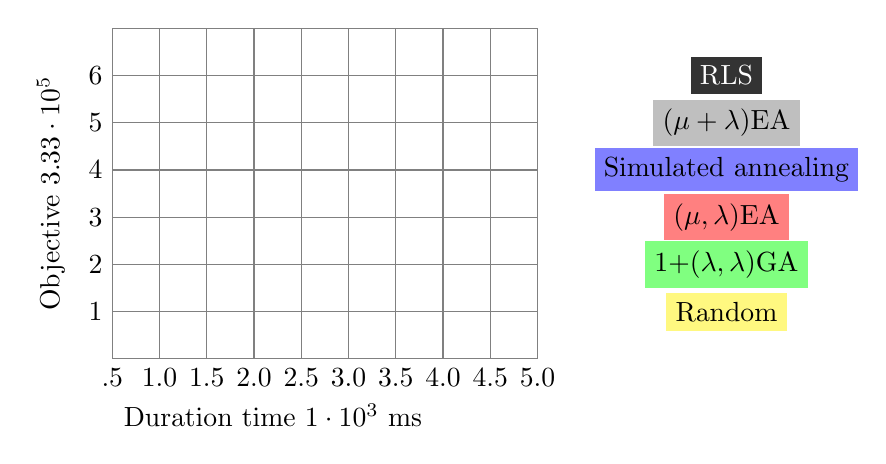
\begin{tikzpicture}[scale = 0.6]
			\draw[step=1,gray,thin]  (0,0) grid (9,7);
			\foreach \x in {.5,1.0,1.5,2.0,2.5,3.0,3.5,4.0,4.5,5.0}
		 \node[anchor=north] at (2*\x-1,0) {\x};
			\foreach \y in {1,2,3,4,5,6}
		 \node[anchor=east] at (0,\y) {\y};
			\draw (3.4,-1.2) node{Duration time $1\cdot10^3$ ms};
			\draw (-1.3,3.5) node[rotate=90]{Objective $3.33\cdot10^5$};
			
			\draw[thick] plot[mark=*]  file {algo1.txt};
			\draw[thick, color=gray] plot[mark=+] file {algo2.txt};
			\draw[thick, color=blue] plot[mark=x] file {algo3.txt};
			\draw[thick, color=red] plot[mark=*] file {algo4.txt};
			\draw[thick, color=green] plot[mark=+] file {algo5.txt};
			\draw[thick, color=yellow] plot[mark=x] file {algo6.txt};
			
			\draw[white] (13,6)node[fill=black!80] {RLS};
			\draw(13,5)node[fill=gray!50] {($\mu+\lambda$)EA};
			\draw(13,4)node[fill=blue!50] {Simulated annealing};
			\draw(13,3)node[fill=red!50] {($\mu,\lambda$)EA};
			\draw(13,2)node[fill=green!50] {1+($\lambda,\lambda$)GA};
			\draw(13,1)node[fill=yellow!50] {Random};
		\end{tikzpicture}
	\end{center}
	\caption{Convergences of different algorithms (basic dataset).}
	\label{expe_convergence}
\end{figure}

\end{document}